\subsection{Mobile Application}
This sub-section describes the design of the OpenWRT remote access mobile application. Since this is a proof of concept, we only designed and implemented the application on Android platform.

\subsubsection{Architecture}
Figure \ref{android-architecture} shows the architecture of the Android OpenWRT remote access application. It contains four modules: the Android activities, network communication module, graphical user interface and response result parser. Among these four modules, the activities combine the other three together to take users' inputs and provide visualized information.

\begin{figure*}
	\centering
	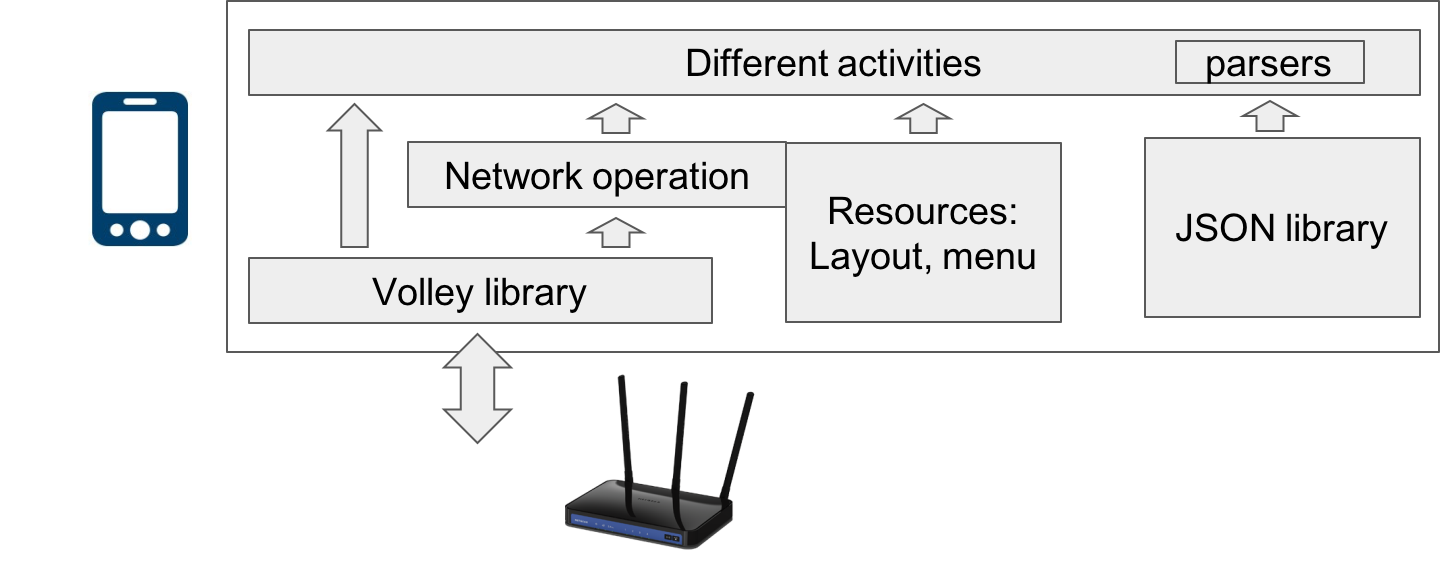
\includegraphics[width=0.75\textwidth]{android-architecture.png}
	\caption{Android application architecture}
	\label{android-architecture}
\end{figure*}

\subsubsection{Network communication}
Since the application needs to communicate with the OpenWRT backend server, it is necessary to provide a network communication module to handle all the network operations, which are shared by activities that need network communications.

LuCI backend and per-application statistics backend both provide http-based interfaces. To commuicate with these two backends, the network communication module needs to be able to send \textit{POST} and \textit{GET} requests and receive responses. A key part is to build proper URLs according to backends' requirements. For example, a \textit{POST} request to communicate with LuCI backend is ``http://<IP address of the OpenWrt Box>:<server port>/cgi-bin/luci/;stok=<stok id>'', and a \textit{GET} request to communicate with per-application statistics backend is ``http://<IP address of the OpenWrt Box>:<server port>/output.txt''.

\subsubsection{Graphical user interface}
The goal of the graphical user interface design was to simplify the user interface on a smartphone. To that end, the limitations of the LuCI web interface were studied to provide design guidelines. The first issue analyzed was that LuCI had an issue in its navigation on smartphones. To navigate through the application categories, the user needed to select a category in the navigation menu, then select a subcategory from the dropdown menu. Additionally, changing subcategories within the same category still required selecting the overarching category again. Therefore, a design goal of the application would be to maintain the current category and simply swap subcategories.
	
Another LuCI WebView issue was that unsaved changes would be tracked in a session until committed. Tracking unsaved changes on a web browser can result in session complications, depending on browser settings for caching. Furthermore, the WebView relied on in-browser scripting to provide functional elements, which is a dependency that can be optimized. Therefore another aspect of our design was to make all actions atomic and contained to the screen they are accessed on, to avoid carrying changes. To make all actions atomic, all functional elements in the original WebView would be rebuilt natively in Android.
	
Based on the LuCI framework, the designed Android application's user interface screens consisted of a login screen, then three major categories: status, network, and system. Each category then presented a subnavigation menu that persisted until another major category was selected, allowing users to move more freely within same category.

	\begin{figure}
		\centering
		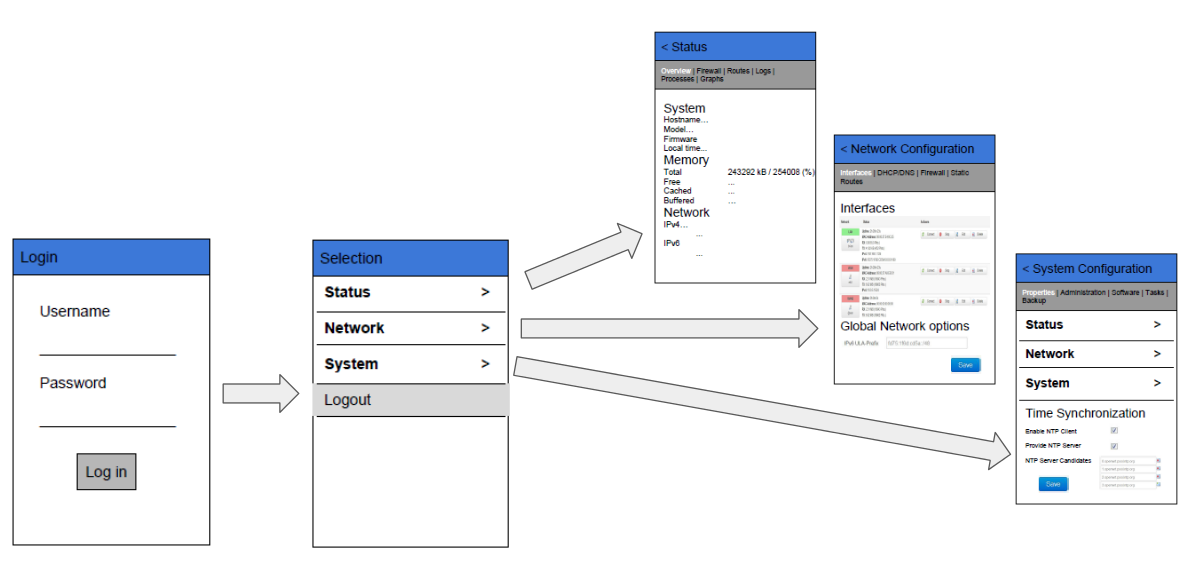
\includegraphics[width=0.4\textwidth]{UItopdown.png}
		\caption{the topdown navigation of the Android GUI design}
		\label{OpenWRT:androidtopdown}
	\end{figure}
	
Each separate screen in the subcategories of the major categories was designed to maintain discrete actions and information. Rather than having multiple configuration forms and submission buttons in the same screen, the screen would be limited to at most one form each, with other forms being accessible on a new screen that is linked to by a list on the current screen.

	\begin{figure}
		\centering
		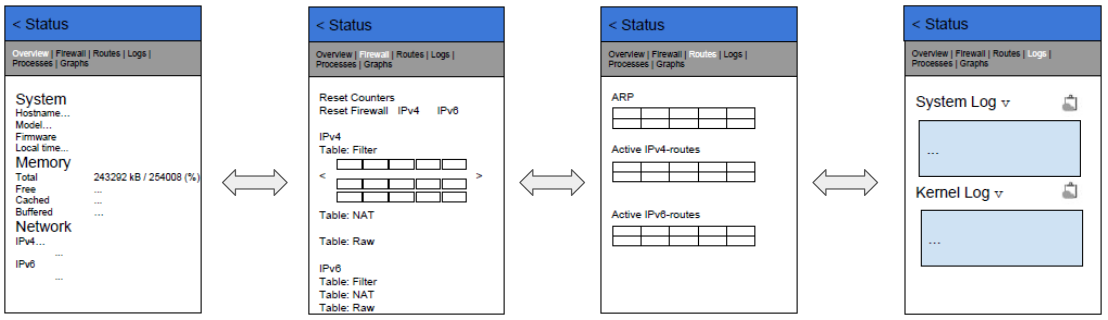
\includegraphics[width=0.4\textwidth]{UIstatus.png}
		\caption{the Android status interfaces}
		\label{OpenWRT:androidstatus}
	\end{figure}
	
	\begin{figure}
		\centering
		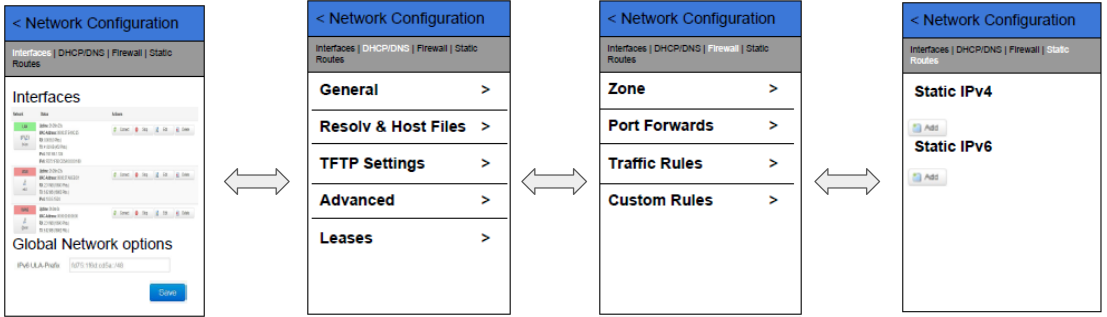
\includegraphics[width=0.4\textwidth]{UInetwork.png}
		\caption{the Android network interfaces}
		\label{OpenWRT:androidnetwork}
	\end{figure}
	\begin{figure}
		\centering
		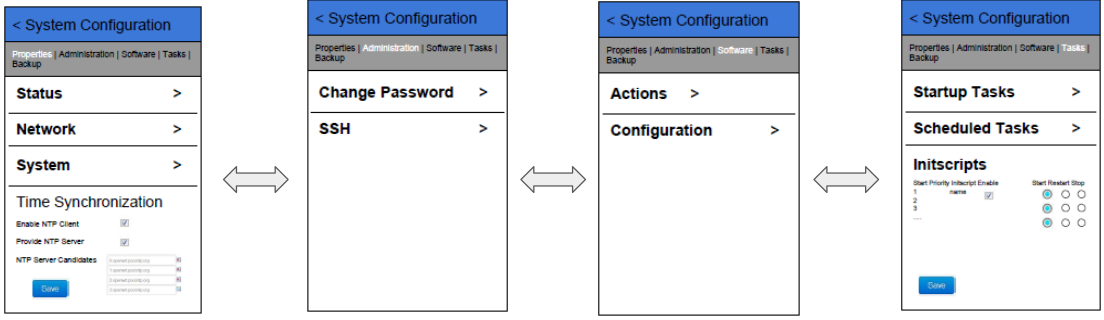
\includegraphics[width=0.4\textwidth]{UIsystem.png}
		\caption{the Android system interfaces}
		\label{OpenWRT:androidsystem}
	\end{figure}

\subsubsection{Network Respond Parser}

After the mobile application sends http requests to the OpenWRT backend, it will get responses. The responses are either an html script or a JSON object. We can parse the html script or JSON object to extract the needed information and fill it into the designed UI. However, such operations takes time on the phone. As a proof of concept, the initial implementation uses Android's WebView class to visualize html scripts.

